
%(BEGIN_QUESTION)
% Copyright 2006, Tony R. Kuphaldt, released under the Creative Commons Attribution License (v 1.0)
% This means you may do almost anything with this work of mine, so long as you give me proper credit

Calculate the hydrostatic pressure generated at the bottom of this vessel (in units of bar) when it is completely filled with water:

$$\includegraphics[height=6cm]{i00308x01.eps}$$

Now calculate the hydrostatic pressure at the bottom of this vessel (in units of bar) when it is completely filled with gasoline (density = 672.8 kg/m$^{3}$):

$$\includegraphics[height=6cm]{i00308x02.eps}$$

\filbreak

What do you think the pressure will be at the bottom of the vessel if it is exactly half-full of gasoline and half-full of water, with a gasoline-water {\it interface} at the 5.5 meters mark?  Explain your reasoning.

$$\includegraphics[height=6cm]{i00308x03.eps}$$

\underbar{file i00308}
%(END_QUESTION)





%(BEGIN_ANSWER)

Hydrostatic pressure when completely full of water = 1.065 bar

\vskip 10pt

Hydrostatic pressure when completely full of gasoline = 0.717 bar

\vskip 10pt

Hydrostatic pressure when water-gasoline interface is at the 50\% level = 0.891 bar


%(END_ANSWER)





%(BEGIN_NOTES)

\vfil \eject

\noindent
{\bf Summary Quiz:}

Calculate the hydrostatic pressure at the bottom of this open vessel, holding 7 feet of gasoline over 6 feet of water:

$$\includegraphics[width=15.5cm]{i00308x04.eps}$$

\begin{itemize}
\item{} 190.9 inches W.C.
\vskip 5pt 
\item{} 105.0 inches W.C.
\vskip 5pt 
\item{} 130.5 inches W.C.
\vskip 5pt 
\item{} 128.5 inches W.C.
\vskip 5pt 
\item{} 132.5 inches W.C.
\vskip 5pt 
\item{} 156.0 inches W.C.
\end{itemize}


%INDEX% Physics, static fluids: hydrostatic pressure of liquid/liquid interface

%(END_NOTES)


